%----------------------------------------------------------------------------------------
%	Inställningar och dokumentkonfiguration
%----------------------------------------------------------------------------------------

\documentclass[paper=a4, fontsize=11pt]{report} % A4-sida och 11 punkters fontstorlek

\usepackage[T1]{fontenc} % 8-bitarskodning som har 256 glyfer
\usepackage[english]{babel} % Svenskt språk(ändrat till engelska)
\usepackage[utf8]{inputenc} % För svenska tecken
\usepackage{dtk-logos} % Logos
\usepackage{wallpaper} % Bakgrundsbild
\usepackage{fancyhdr} % Specialsidhuvud och sidfot
\usepackage{enumerate} 
\usepackage{hyperref}
\usepackage{textcomp}
\usepackage{xifthen}% provides \isempty test
\pagestyle{fancyplain} % Använd sidhuvud och sidfot på alla sidor
\fancyhead[L]{Laboration 2 -- 1DV720 -- \the\year -- Server administration} % Titel till vänster i sidhuvud
\fancyhead[C]{} % Tomt i mitten
\fancyhead[R]{} % Tomt till höger
\fancyfoot[L]{{\color{gray}\textcopyright \ \the\year \ Jacob Lindehoff}} % Tomt till vänster
\fancyfoot[C]{}  % Tomt i mitten
\fancyfoot[R]{\thepage} % Sidnumrering till höger i sidfoten
\renewcommand\thesection{\arabic{section}} % Section beter sig som i dokumentklassen article

\newcommand{\win}[1]{Microsoft Windows Server\ifthenelse{\isempty{#1}}{}{ #1}}
\newcommand{\gui}[0]{``Server with a GUI''}
\newcommand{\core}[0]{Windows Server Core}
%----------------------------------------------------------------------------------------
%	TITLE SECTION
%----------------------------------------------------------------------------------------
\newcommand\BackgroundPic{
    \put(-50,-50){
    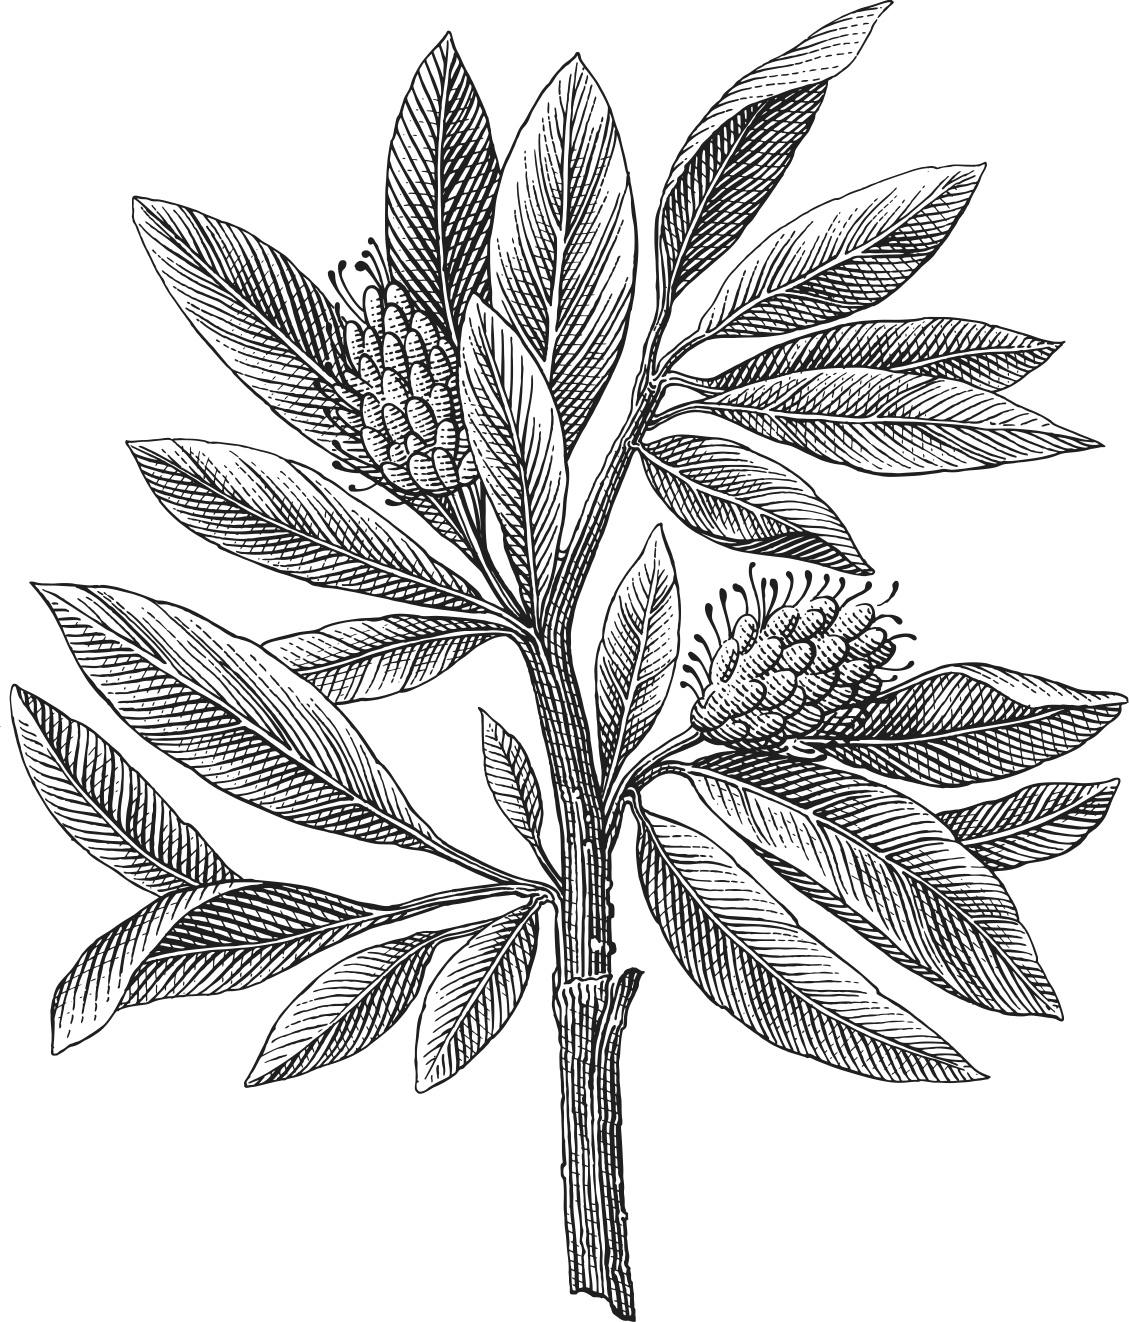
\includegraphics[keepaspectratio,scale=0.65]{lnu_etch.png} % Bakgrundsbild
    }
}
\newcommand\BackgroundPicLogo{
    \put(15,700){
    
\includegraphics[keepaspectratio,scale=0.10]{logo.png} % Logga i vänstra hörnet
    }
}

\newcommand{\horrule}[1]{\rule{\linewidth}{#1}} % Skapa hortisontell linje

\title{	\vspace{-10cm}
    \normalfont \normalsize
    \textsc{Linnaeus University} \\ [25pt] % Universitetes namn
    \horrule{0.5pt} \\[0.4cm] % Tunn linje högst upp
    \huge Laboration 2\\ % Arbetes titel
	\large \textcolor{gray}{1DV720 -- Server Administration}
    \horrule{0.5pt} \\[0.4cm] % Tunn linje längst ner
}

% \author{Jacob Lindehoff} % Författarnas namn

\date{\normalsize\today} % Dagens datum

\begin{document}
\AddToShipoutPicture*{\BackgroundPic} % Lägger in backgrundsbild på första sidan
\AddToShipoutPicture*{\BackgroundPicLogo}
\maketitle % Skriv ut titeln
\noindent % Tabba inte in på första meningen

%------------------------------------------------
%	Introduction
%------------------------------------------------
\section{Introduction}

For this lab we will look into filesystems, partitioning, permissions and how these can be applied in a server environment. We will modify the lab environment, you can reuse some machine or start from scratch and delete all machines from lab 1. Before you delete any machine make sure that you have passed Lab 1.

\pagebreak
%------------------------------------------------
%	Uppgift
%------------------------------------------------
\section{Assignment}
\begin{figure}[h]
\centering
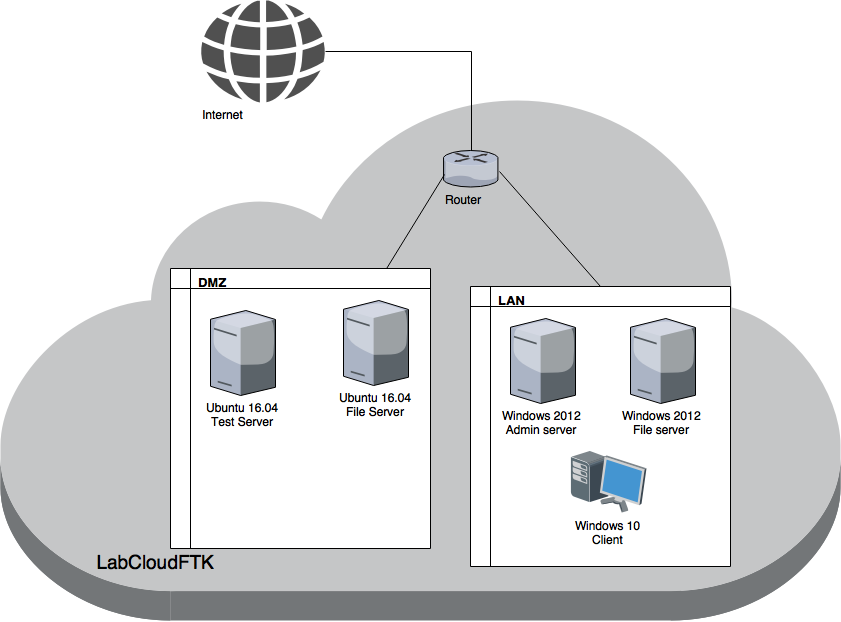
\includegraphics[width=1\linewidth]{./Lab02-Network}
\caption[Figure over network in Lab 2]{The network as it should be setup in Lab 2.}
\label{fig:network}
\end{figure}
Now that you have set up the basic network and made sure the machines can communicate, it's time to move on and configure some file servers. In \figurename \ref{fig:network} you should see how the network should look when you are done with lab 2.

The topology contains two separated networks, one is for the internal network witch shouldn't be be able to contact from the outside. The other network is for servers that should be publicly access like Web servers and Name servers. In the internal network called LAN you should have three machines, one Admin Server from where you will manages all of the machine both in the LAN and the DMZ. The second server in the LAN should be a Windows file server and the last machine is a client machine that will be used to test the permissions on the file server. In the second network, DMZ, you should have two Linux server. One file server, that later on will be used for the web servers, and one server to test connectivity and permissions of the file server.

\pagebreak

\section{Requirements}
\label{tasks}
As in the first lab, security is important and all machines should have there firewalls enabled. Firewall rules will be checked to be ‘decent’. Remember that if (as it should be) your firewall is properly setup you will need to make exception for the protocols you are implementing.
As previously your configuration should survive a reboot.

\begin{itemize}
    \item All machines should:
    \begin{itemize}
		\item should have internet access
		\item within the same network be able to ping each other
		\item not be able to contact each other if not in the same network, except for the Admin Server
        \item have proper firewall rules. This includes both the linux and windows machines
    	\item have a proper naming convention.
    \end{itemize}
	\item Specific machine requirements:
    \begin{itemize}
        \item \textbf{LAN} - Admin Server
        \begin{itemize}
			\item OS: Windows Server 2012 R2 \textbf{GUI}
			\item This is the only machine that should be able to contact from Internet using RDP
			\item Only RDP traffic should be allowed from Internet
        	\item It should have an strong an complex password.
        	\item You should be able to manage other servers/clients, both in LAN and DMZ, from this machine using SSH and RDP
        \end{itemize}        
        \item \textbf{LAN} - File Server
        \begin{itemize}
			\item OS: Windows Server 2012 R2 \textbf{Core}
			\item should have 3 volume connected to it that should be configured as one volume with RAID 5 and formatted with NTFS. \textbf{Only use 1 GB volumes}.
			\item this new volume should have a shared folder with different permissions for different users
			\item you should have at least 3 different users with different file permissions on the share, they should not have access to other parts of the server.
        \end{itemize}
        \item \textbf{LAN} - Windows Client
        \begin{itemize}
			\item OS: Windows 10
			\item should be able to connect to the file server
			\item you should be able to login with have at least 3 different users that should have different file permissions on the file server
        \end{itemize}
        \item \textbf{DMZ} - File server
        \begin{itemize}
			\item OS: Ubuntu 16.04
			\item should have one extra volume configured and formatted with an appropriate file system
			\item this volume should be used to share a folder with NFS
			\item only the Test server should be able to connect to the shared folder
        \end{itemize}
        \item \textbf{DMZ} - Test server
        \begin{itemize}
			\item OS: Ubuntu 16.04
			\item should have the file server share mounted
        \end{itemize}  
    \end{itemize}
\end{itemize}

\section{Work Environment}
\label{environment}

You will be using FTK Lab Cloud to be able to accomplish this lab. You will find your credentials and tutorial on how to get started on this page: \href{https://coursepress.lnu.se/kurs/serveradministration/lab-cloud/}{https://coursepress.lnu.se/kurs/serveradministration/lab-cloud/}

For this lab I have also created a video tutorial on how to set up an admin server and the basics for this lab. You'll find it on the \texttt{\href{https://coursepress.lnu.se/kurs/serveradministration/moduler/module-2/laboration}{course homepage}}.


\end{document}
